\begin{figure}[h] 
\centering 
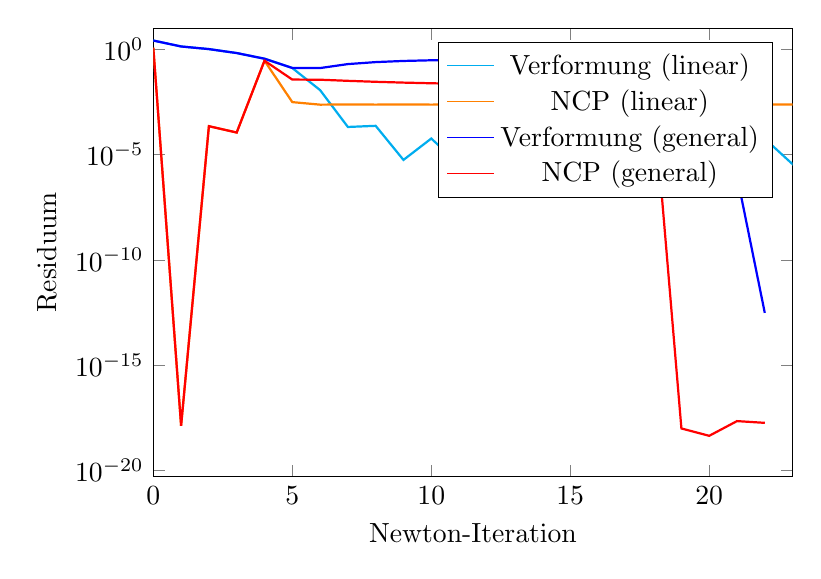
\begin{tikzpicture}[every plot/.append style={thick}] 
\begin{axis}[ 
label style={font=\normalsize}, 
xlabel={Newton-Iteration}, 
ylabel={Residuum}, 
xmin=0, xmax=23, 
ymode=log, 
ymin=0, ymax=10, 
width=0.8\textwidth, 
height=0.6\textwidth, 
legend pos=north east, 
legend style={cells={align=left}}, 
grid style=dashed, 
] 
\addplot[ 
color=cyan, 
] 
coordinates { 
(0, 2.60e+00)(1, 1.36e+00)(2, 1.02e+00)(3, 6.62e-01)(4, 3.56e-01)(5, 1.29e-01)(6, 1.15e-02)(7, 2.04e-04)(8, 2.31e-04)(9, 5.55e-06)(10, 5.75e-05)(11, 3.49e-06)(12, 5.62e-05)(13, 3.47e-06)(14, 5.61e-05)(15, 3.47e-06)(16, 5.61e-05)(17, 3.47e-06)(18, 5.61e-05)(19, 3.47e-06)(20, 5.61e-05)(21, 3.47e-06)(22, 5.61e-05)(23, 3.47e-06)(24, 5.61e-05)(25, 3.47e-06)(26, 5.61e-05)(27, 3.47e-06)(28, 5.61e-05)(29, 3.47e-06)(30, 5.61e-05)(31, 3.47e-06)(32, 5.61e-05)(33, 3.47e-06)(34, 5.61e-05)(35, 3.47e-06)(36, 5.61e-05)(37, 3.47e-06)(38, 5.61e-05)(39, 3.47e-06)(40, 5.61e-05)(41, 3.47e-06)(42, 5.61e-05)(43, 3.47e-06)(44, 5.61e-05)(45, 3.47e-06)(46, 5.61e-05)(47, 3.47e-06)(48, 5.61e-05)(49, 3.47e-06)(50, 5.61e-05)(51, 3.47e-06)(52, 5.61e-05)(53, 3.47e-06)(54, 5.61e-05)(55, 3.47e-06)(56, 5.61e-05)(57, 3.47e-06)(58, 5.61e-05)(59, 3.47e-06)(60, 5.61e-05)(61, 3.47e-06)(62, 5.61e-05)(63, 3.47e-06)(64, 5.61e-05)(65, 3.47e-06)(66, 5.61e-05)(67, 3.47e-06)(68, 5.61e-05)}; 
\addlegendentry{Verformung (linear)} 
\addplot[ 
color=orange, 
] 
coordinates { 
(0, 1.20e+00)(1, 1.30e-18)(2, 2.22e-04)(3, 1.11e-04)(4, 2.86e-01)(5, 3.09e-03)(6, 2.34e-03)(7, 2.39e-03)(8, 2.35e-03)(9, 2.39e-03)(10, 2.35e-03)(11, 2.39e-03)(12, 2.35e-03)(13, 2.39e-03)(14, 2.35e-03)(15, 2.39e-03)(16, 2.35e-03)(17, 2.39e-03)(18, 2.35e-03)(19, 2.39e-03)(20, 2.35e-03)(21, 2.39e-03)(22, 2.35e-03)(23, 2.39e-03)(24, 2.35e-03)(25, 2.39e-03)(26, 2.35e-03)(27, 2.39e-03)(28, 2.35e-03)(29, 2.39e-03)(30, 2.35e-03)(31, 2.39e-03)(32, 2.35e-03)(33, 2.39e-03)(34, 2.35e-03)(35, 2.39e-03)(36, 2.35e-03)(37, 2.39e-03)(38, 2.35e-03)(39, 2.39e-03)(40, 2.35e-03)(41, 2.39e-03)(42, 2.35e-03)(43, 2.39e-03)(44, 2.35e-03)(45, 2.39e-03)(46, 2.35e-03)(47, 2.39e-03)(48, 2.35e-03)(49, 2.39e-03)(50, 2.35e-03)(51, 2.39e-03)(52, 2.35e-03)(53, 2.39e-03)(54, 2.35e-03)(55, 2.39e-03)(56, 2.35e-03)(57, 2.39e-03)(58, 2.35e-03)(59, 2.39e-03)(60, 2.35e-03)(61, 2.39e-03)(62, 2.35e-03)(63, 2.39e-03)(64, 2.35e-03)(65, 2.39e-03)(66, 2.35e-03)(67, 2.39e-03)(68, 2.35e-03)}; 
\addlegendentry{NCP (linear)} 
\addplot[ 
color=blue, 
] 
coordinates { 
(0, 2.60e+00)(1, 1.36e+00)(2, 1.02e+00)(3, 6.62e-01)(4, 3.56e-01)(5, 1.29e-01)(6, 1.28e-01)(7, 1.98e-01)(8, 2.46e-01)(9, 2.79e-01)(10, 3.00e-01)(11, 3.12e-01)(12, 3.15e-01)(13, 3.15e-01)(14, 3.15e-01)(15, 3.09e-01)(16, 3.12e-01)(17, 2.50e-01)(18, 2.17e-01)(19, 9.84e-02)(20, 1.86e-03)(21, 9.75e-07)(22, 3.00e-13)}; 
\addlegendentry{Verformung (general)} 
\addplot[ 
color=red, 
] 
coordinates { 
(0, 1.20e+00)(1, 1.30e-18)(2, 2.22e-04)(3, 1.11e-04)(4, 2.86e-01)(5, 3.64e-02)(6, 3.58e-02)(7, 3.17e-02)(8, 2.85e-02)(9, 2.61e-02)(10, 2.43e-02)(11, 2.28e-02)(12, 2.17e-02)(13, 2.04e-02)(14, 1.78e-02)(15, 1.56e-02)(16, 1.27e-02)(17, 9.52e-03)(18, 4.76e-03)(19, 9.70e-19)(20, 4.34e-19)(21, 2.17e-18)(22, 1.79e-18)}; 
\addlegendentry{NCP (general)} 
\end{axis} 
\end{tikzpicture} 
\caption{Residuen des Stoffgesetzes 'St.Venant' mit Hinderniss 'Hut' und 162 Freiheitsgraden für die Verschiebung.} 
\label{fiq:St.Venant_Hut_level2} 
\end{figure} 
